\chapter{Introduction}
This report and the corresponding documentation with its appendix is written as the documentation for the process of the developing the AU2 car, the dynamometer dubbed Rolling Road and the GUI developed for use with the Rolling Road. The products being developed are made to compete in the Shell Eco Marathon. The proces of the development is made in correlation with Aarhus School of Engineering(ASE). The development is part of the 4. semester project. 

This report covers three major subjects:

\begin{itemize}
	\item{AU2}
	\item{Rolling Road}
	\item{GUI}
\end{itemize}

AU2 is the car made for the competing in the Shell Eco Marathon. In this report the electrical systems made for controlling the car will be described. For more information containing calculations and general informations about the physcial implementation of the car please visit the technical documentation on this.

The Rolling Road and GUI is a coherent system, though they can work independently. This report will only cover the electrical system developed along with the software, both for Rolling Road and the GUI. 

This report will only scratch the surface. For in-depth design and implementation features, please visit the associated documentation. 

The products being developed will serve as a working product that has been thoroughly tested. This is done so that no breakdown occurs during the race. It will also work as a guideline for future work for other students and therefore it is necessary that the documentation provided alongside this report must be comprehensive.

\section{List of terms}
Text

\section{Reading guide}
Read it

\section{Areas of responsibility}
In the following table the teammembers will describe their primary responsibilities during the project. 

\begin{tabular}[c]{|p{3cm}| p{5cm} | p{6cm}|}
	\hline
	\textbf{Member} & \textbf{Area of responsibility} & \textbf{Description}\\\hline
	
	% Jens
	\phantom{Test}
	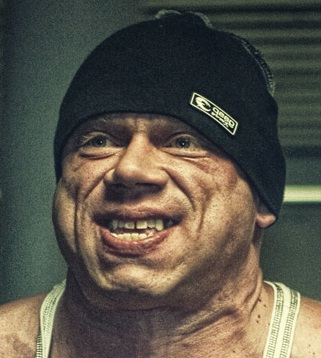
\includegraphics[width=3cm]{Introduction/TeamPictures/Jens} & \multirow{2}{5cm}{Area of responsibility goes here} & \multirow{2}{6cm}{Description goes here plzzzzzzzzzzzzzzzz} \\
	Jens P. Nymann & & \\ \hline
	
	%Jonas
	\phantom{Test}
	
\includegraphics[width=3cm]{Introduction/TeamPictures/Jonas} & \multirow{2}{5cm}{Area of responsibility goes here} & \multirow{2}{6cm}{Description goes here plzzzzzzzzzzzzzzzz} \\
	Jonas M. Hansen & & \\ \hline
	
	%Jonathan
	\phantom{Test}
	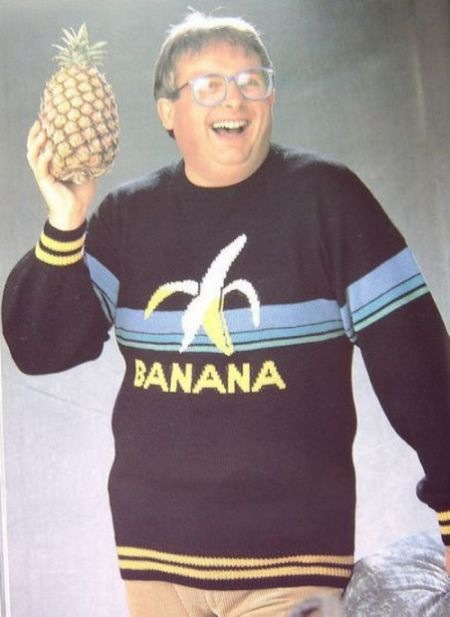
\includegraphics[width=3cm]{Introduction/TeamPictures/Jonathan} & \multirow{2}{5cm}{Area of responsibility goes here} & \multirow{2}{6cm}{Description goes here plzzzzzzzzzzzzzzzz} \\
	Jonathan Schougaard & & \\ \hline
\end{tabular}

\newpage
\begin{tabular}[c]{|p{3cm}| p{5cm} | p{6cm}|}
	\hline
	\textbf{Member} & \textbf{Area of responsibility} & \textbf{Description}\\\hline
	
	%Laimonas
	\phantom{Test}
	
\includegraphics[width=3cm]{Introduction/TeamPictures/Laimonas} & \multirow{2}{5cm}{Area of responsibility goes here} & \multirow{2}{6cm}{Description goes here plzzzzzzzzzzzzzzzz} \\
	Laimonas I. \newline Bendikas & & \\ \hline
		
	%Thomas R
	\phantom{Test}
	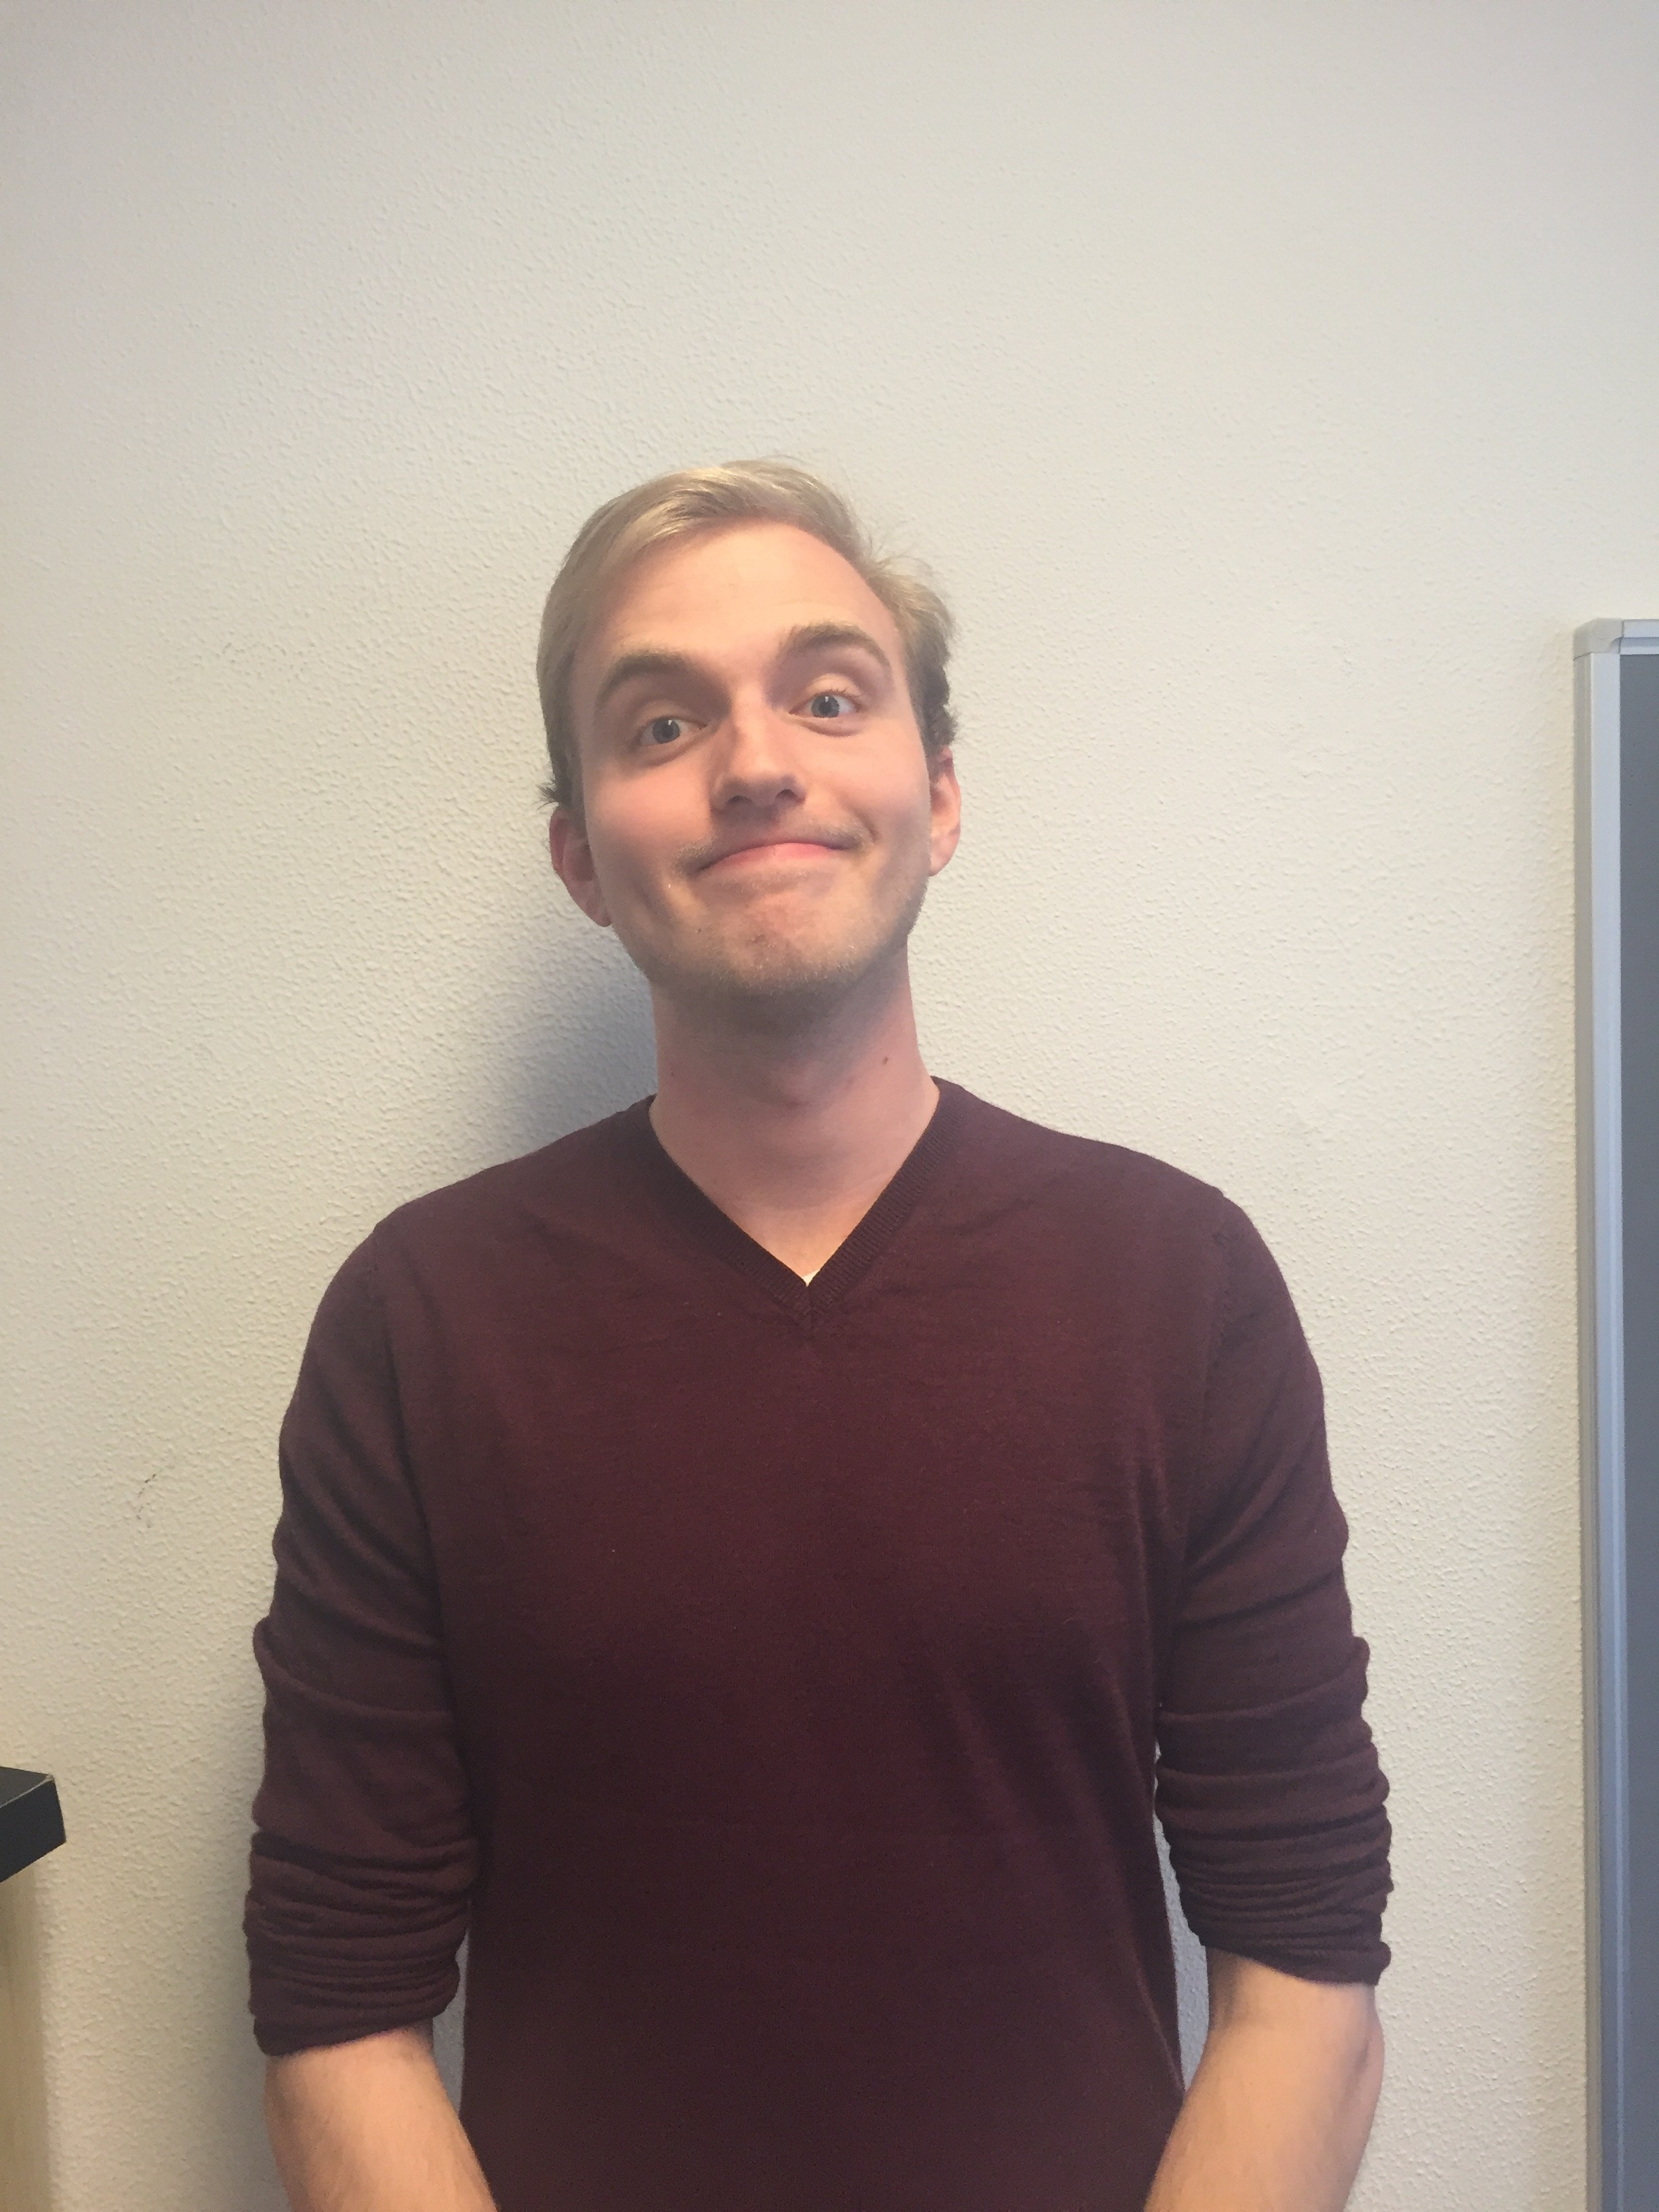
\includegraphics[width=3cm]{Introduction/TeamPictures/ThomasR} & \multirow{2}{5cm}{Area of responsibility goes here} & \multirow{2}{6cm}{Description goes here plzzzzzzzzzzzzzzzz} \\
	Thomas S. \newline Rasmussen & & \\ \hline
		
	%Thomas N
	\phantom{Test}
	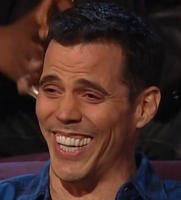
\includegraphics[width=3cm]{Introduction/TeamPictures/ThomasN} & \multirow{2}{5cm}{Hardware development for AU2 and protocol development for RR} & \multirow{2}{6cm}{I have been responsible for the design and implementation of the hardware for AU2. Furthermore I have developed the Protocol for Rolling Road} \\
	Thomas B. \newline Nielsen & & \\ \hline
\end{tabular}